\chapter{Design and Implementation}
\label{ch:design_implementation}
This chapter describes the design and implementation of the delegation mechanisms integrated into vodle, detailing both the technical approach and practical decisions made throughout development. It begins by outlining vodle's existing system architecture, clarifying how this influenced the integration of new delegation features. 

Each subsequent section aligns directly with one of the project objectives defined previously, explaining the rationale behind key design choices, algorithms, and interface elements. Emphasis is placed on the critical design trade-offs and challenges encountered, highlighting how constraints such as the serverless architecture and client-side computation informed implementation decisions.

\section{System Architecture Overview}\label{sec:design_architecture}
Vodle is built as a serverless web application that emphasises accessibility, client-side performance, and ease of deployment. Its architecture comprises two components:

\begin{enumerate}
  \item \textbf{Frontend:} Implemented using Angular and the Ionic framework, the frontend provides a responsive and modular interface that works across both desktop and mobile devices. The use of Angular facilitates the creation of component-based user interfaces, essential for introducing interactive features such as the ranked delegation UI and vote splitting sliders.
  \item \textbf{Backend:} Vodle uses CouchDB as its database. There is no custom backend logic or middleware; instead, the frontend application communicates directly with CouchDB over HTTP.
\end{enumerate}

\subsubsection{Implications of This Architecture}
Vodle's serverless architecture has several implications for the design and implementation of the delegation mechanisms, especially due to the absence of a traditional data processing backend. The following points summarise the key considerations:
\begin{itemize}
  \item All vote delegation logic, including transitive resolution, cycle detection, and vote splitting calculations, must be executed in the browser. This places constraints on performance and requires careful optimisation of algorithms used.
  \item CouchDB's document-based storage model means that all data must be serialised and deserialised in JSON format. This affects how data structures are designed and manipulated, as well as how they are stored and retrieved from the database.
\end{itemize}

\subsection{CouchDB Storage and Write Constraints}
\label{subsec:couchdb_limits}

Vodle store all data in CouchDB in two types of databases: the \_users database and poll databases. The \_users database is a standard CouchDB database that stores user documents, while the poll databases are created dynamically for each poll and contain all relevant data for that poll.

\begin{enumerate}
  \item \textbf{\_users Database.}
    \begin{itemize}
      \item Each document ID is \texttt{org.couchdb.user:<username>}.
      \item Only the account owner or an administrator may modify or delete their user document.
    \end{itemize}

  \item \textbf{Poll Databases.}
    \begin{itemize}
      \item Databases are named \texttt{poll-<POLLID>}.
      \item Stores:
        \begin{itemize}
          \item The immutable poll definition (\texttt{poll.json}).
          \item One vote document per voter (\texttt{vote-<user>}).
        \end{itemize}
    \end{itemize}
\end{enumerate}

\paragraph{Document-Level Security}
CouchDB enforces security at the level of entire documents. This means that access control decisions are made based on the identity of the user attempting to write a document and the document's ID -- there is no support for restricting access to individual fields within a document. Additionally, CouchDB does not support merging concurrent changes; updates must replace the entire document in a single write operation. As a result, all write operations are either fully accepted or fully rejected by the database's \texttt{validate\_doc\_update} function. This strict model simplifies validation logic but introduces important constraints in the context of implemented liquid democracy, which are discussed in the remainder of this section.

\subsubsection{Poll-DB Validation}
When a client writes to a poll database, the \texttt{validate\_doc\_update} enforces:

\begin{enumerate}
  \item \textbf{User Documents:} IDs are prefixed with \texttt{~vodle.user.}, and only the owner may modify them:
\begin{figure}[H]
  \centering
\begin{minted}{typescript}
if (!id.startsWith(`~{userCtx.name}§`)) {
  throw({ forbidden: 'Only the document owner may modify this user doc.' });
}
\end{minted}
\caption{Code to prevent a user from modifying another user's document.}
\end{figure}

  \item \textbf{Immutable Poll Artefacts: } Documents like \texttt{poll.json} or results cannot be updated once created:
\begin{figure}[H]
    \begin{minted}[fontsize=\small,baselinestretch=1]{javascript}
if (oldDoc && isPollArtifact(id)) {
  throw({ forbidden: 'Poll documents are immutable once created.' });
}
    \end{minted}
\caption{Code to prevent modification of poll artefacts.}
\end{figure}
\end{enumerate}

\subsubsection{\_users-DB Validation}
In the \_users database, a similar validation function is used to prevent users from modifying other users' documents, including the \texttt{vodle} service account.
\begin{figure}[H]
\begin{minted}[fontsize=\small,baselinestretch=1]{javascript}
if (id !== `org.couchdb.user:{userCtx.name}`) {
  throw({ forbidden: 'Users may only modify their own user document.' });
}
if (userCtx.name === 'vodle' || isPollService(userCtx.name)) {
  throw({ forbidden: 'Service accounts are immutable.' });
}
\end{minted}
\caption{Code to prevent a user from modifying another user's document.}
\end{figure}

\subsection{Summary of Storage and Validation Constraints}
\label{subsec:summary_storage_constraints}

The architecture of vodle, particularly its reliance on CouchDB and the absence of a custom backend, imposes important constraints on how delegation features are designed and implemented.

\begin{itemize}
  \item \textbf{User autonomy is strictly enforced.} Each user can only modify documents that are explicitly associated with their own identity. This guarantees that vote and delegation data cannot be tampered with by other clients but also eliminates the possibility of directly setting or managing another user's vote.

  \item \textbf{Issues with sharing a document.} The current database design does not support the modification of a single document by multiple users. As a result, features that require a global view -- such as a delegation graph -- require a rework of the database schema.

  \item \textbf{Validation logic is structural, not contextual.} Since CouchDB validation functions can only inspect the document being written, they cannot reason about relationships across documents. This prohibits logic such as resolving delegations server-side, enforcing uniqueness of votes, or validating delegation cycles at the point of write.

  \item \textbf{Client-side logic carries the burden.} Due to the point above, all logic for delegation resolution, cycle checking, and vote splitting must be implemented in the client. This requires careful design to ensure that the frontend can handle complex delegation scenarios without overwhelming the user or causing performance issues.
\end{itemize}

Together, these constraints shape some of the design and implementation choices of the delegation features in vodle, which will be discussed in detail in the following sections.

\section{Implement a Core Delegation Model into vodle}
\label{sec:core_delegation_detailed}
This section describes the design and implementation of the core delegation mechanism in vodle, which allows users to delegate their votes to others. It covers the issues with the original implementation and the challenges solved in the redesign.

\subsection{Existing Delegation Interaction Flow}
Figure~\ref{fig:delegation-flow-accept} depicts the life-cycle of a delegation. The diagram is intentionally simple--only the four message exchanges required to set up or tear down a delegation are shown--so the reader can map each arrow to a concrete API call or UI control.

% ------------- DIAGRAM PLACEHOLDER -------------
% Replace the TikZ skeleton with an exported SVG once finalised.
\begin{figure}[H]
  \centering
  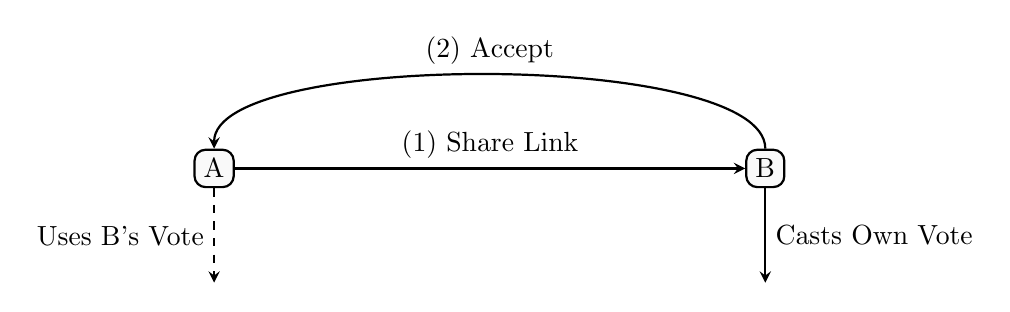
\begin{tikzpicture}[node distance=7cm,>=stealth,thick]
    % clients
    \node[rectangle,draw,rounded corners,fill=gray!5] (A) {A};
    \node[rectangle,draw,rounded corners,fill=gray!5,right of=A] (B) {B};
    % arrows
    \draw[->] (A) -- node[above]{(1) Share Link} (B);
    \draw[->] (B) .. controls +(0,1.5) and +(0,1.5) .. node[above]{(2) Accept} (A);
    \draw[->] (B.south) -- ++(0,-1.2) node[midway,right]{Casts Own Vote};
    \draw[->, dashed] (A.south) -- ++(0,-1.2) node[midway,left]{Uses B's Vote};
  \end{tikzpicture}
  \caption{Sequence for a delegation to be initiated. User A shares a link with user B, who accepts the delegation.}
  \label{fig:delegation-flow-accept}
\end{figure}

\begin{figure}[H]
  \centering
  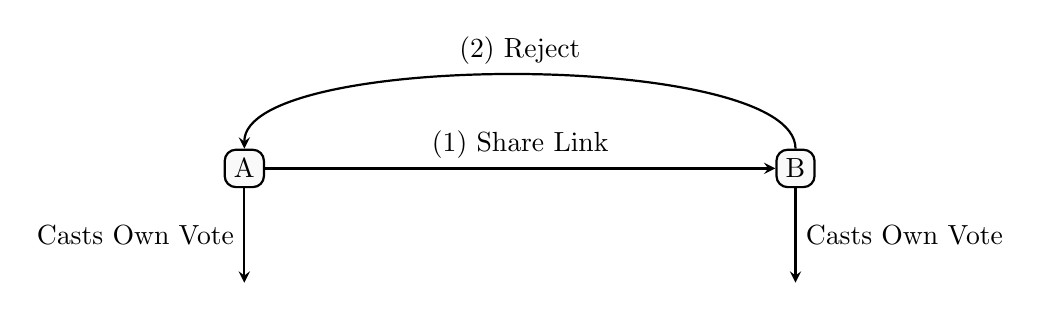
\begin{tikzpicture}[node distance=7cm,>=stealth,thick]
    % clients
    \node[rectangle,draw,rounded corners,fill=gray!5] (A) {A};
    \node[rectangle,draw,rounded corners,fill=gray!5,right of=A] (B) {B};
    % arrows
    \draw[->] (A) -- node[above]{(1) Share Link} (B);
    \draw[->] (B) .. controls +(0,1.5) and +(0,1.5) .. node[above]{(2) Reject} (A);
    \draw[->] (B.south) -- ++(0,-1.2) node[midway,right]{Casts Own Vote};
    \draw[->] (A.south) -- ++(0,-1.2) node[midway,left]{Casts Own Vote};
  \end{tikzpicture}
  \caption{Sequence for a rejected delegation. User A shares a delegation link with user B, who rejects the delegation.}
  \label{fig:delegation-flow-reject}
\end{figure}

% \subsection{Issues Prior to Redesign - unnecessary?}
% The original implementation of liquid democracy in vodle functions as a proof-of-concept, but it has several limitations that hinder its usability and reliability. The following sections outline some of the key issues that were identified whilst planning the redesign.

% \textbf{Inconsistency in data between clients} delegation graph not synched -- leads to cycle checking issue \dots

% \paragraph{Out-of-sync state} Each browser session cached its own copy of the delegation graph; no push notifications existed to bring other clients up-to-date.
% \paragraph{Inconsistent cycle checking} Because state diverged, the local "no-loop" tests sometimes produced different answers on different machines.
% \paragraph{UI drift} Controls such as ``delegate none/some/all'' and the ``your vote is used for \(n\) others'' badge used stale data and became misleading.

\subsection{Cycle Checking}
Robust cycle detection is a core requirement for any system implementing transitive delegation. In liquid democracy, cycles render votes unresolved and potentially lost, directly undermining the integrity of the outcome. Given vodle's dynamic and client-driven architecture, it was crucial to implement an efficient, client-side mechanism that could detect and prevent cycles in real time, without requiring server-side intervention or excessive computation.

The original implementation of cycle prevention in vodle was incomplete and inconsistently enforced. Because delegation data was locally cached and not always synchronised across clients, users could unknowingly create cycles that would only be caught (or missed) depending on the state of their browser session. This led to erratic user experiences, where a delegation might succeed on one device but be rejected on another.

The redesigned cycle checking approach addresses this inconsistency through the introduction of a shared data structure, stored in CouchDB and updated collaboratively by all clients. This ensures consistent validation of new delegations and enables immediate feedback to users attempting to create an invalid delegation path. The remainder of this section details the algorithmic choices, data structures, and UI modifications used to implement reliable cycle detection in vodle.

\subsubsection{Algorithm Design}
The current delegations in a system can be represented as a directed graph where each user is represented as a node and each delegation is represented as a directed edge $(u,v)$, where $u$ is the delegator and $v$ is the delegate. The goal of the cycle-checking algorithm is to ensure that a proposed delegation does not create a cycle in this directed graph.

A new delegation $X\to Y$ is valid if and only if $Y$ is \emph{not} reachable from $X$ in that DAG -- if $Y$ is not a descendant of $X$.

Instead of checking for this condition directly using a depth-first search (DFS) or breadth-first search (BFS), a more efficient approach is to maintain a list of all descendants for each user. This allows us to check if $Y$ is in the list of descendants of $X$ in constant time. The implementation of this algorithm is detailed in the next section.

\subsubsection{Implementation Details}
A hashmap is used to store the descendants of each user. The keys are user IDs, and the values are sets of user IDs representing the direct delegates of that user. In the code, this hashmap is referred to as ``\verb|inverse_indirect_map|''.
\begin{figure}[H]
  \centering
  \begin{minted}{json}
    "inverse_indirect_map": {
      "B": ["A"],
      "C": ["B", "A"],
      "D": ["C", "B", "A"]
    }
  \end{minted}
  \caption{Example of a hashmap for users A, B, C, and D. User A has delegated to B, user B has delegated to C, and user C has delegated to D. Consequently, the descendants of user D are A, B and C.}
  \label{fig:inverse_indirect_map}
\end{figure}

This map enables several key operations required for maintaining a consistent and cycle-free delegation graph:

\begin{itemize}
  \item \textbf{Check Delegation Validity:} To determine whether a delegation \(X \!\to\! Y\) would create a cycle, the system checks if \(Y\) already appears in the set of descendants of \(X\). If so, the new delegation is invalid. This check takes \(O(1)\) time.
  \begin{figure}[H]
    \centering
    \begin{minted}{javascript}
      const inverse_indirect_map = this.G.D.get_inverse_indirect_map(pid);
      const descendant_set = inverse_indirect_map.get(delegate_vid);
      if (descendant_set.has(myvid)) {
        cycle = true;
      }
    \end{minted}
    \caption{Code for checking if a delegation is valid. This check is triggered when a user clicks on a delegate link. The map is retrieved from the synchronised local cache, and the set of descendants is used to confirm that a cycle would not be formed.}
  \end{figure}

  \item \textbf{Add Delegation Edge:} When a new delegation \(X \to Y\) is accepted, the system must ensure that the descendant relationship is updated consistently. Specifically, for $Y$ and every user \(u\) such that \(Y \in \texttt{desc}(u)\), their descendants must be updated to include both \(X\) and all of \(X\)'s current descendants.

  \item \textbf{Remove Delegation Edge:} When a delegation \(X \!\to\! Y\) is removed, the system must ensure that the descendant relationship is updated consistently. Specifically, for $Y$ and every user \(u\) such that \(Y \in \texttt{desc}(u)\), their descendants must be updated to remove both \(X\) and all of \(X\)'s current descendants.
\end{itemize}

\subsubsection{Synchronisation -- TODO}
Explain CouchDB problem with poll db and user db. Every user needs to be able to fetch and push \verb|inverse_indirect_map|.

\subsubsection{Practical Challenges -- TODO}

\subsection{User Interface Changes -- TODO}
\begin{itemize}
  \item Re-bound the ``delegate none/some/all'' switch so it toggles \emph{only} the current option and refreshes its label after server confirmation.
  \item Re-implemented the ``vote is used for \(n\) others'' badge so it recomputes from the latest \texttt{inverse\_indirect\_map} rather than client guesses.
  \item Added unobtrusive toast notifications when a delegation request is rejected (e.g.\ cycle detected) so the user can immediately choose another delegate.
\end{itemize}

\subsection{Summary -- TODO}


\section{Implement Ranked Delegation into Vodle}\label{sec:design_ranked_delegation}
This feature introduced ranked delegation using the MinSum rule, allowing users to list fallback delegates in case their primary choice was unavailable.

\begin{itemize}
  \item UI for setting delegate rankings
  \item New UI when making a poll to allow user to select ranked delegation.
  \item \verb|direct_delegation_map|: maps user IDs to list of ranked delegates [[delegationid, rank, status]...]
  \item Explanation and application of the MinSum rule
  \item How do we determine who is a casting voter?
  \item Implementation of ranked path resolution
  \item Illustrations and code snippets
\end{itemize}

\subsubsection{Challenges}
The MinSum rule had to be implemented efficiently using only browser-based resources. Ranking resolution had to preserve user intent while avoiding delegation ambiguity. Providing visual feedback to help users understand how rankings would resolve added an additional layer of design complexity.

\section{Implement a Vote Splitting Delegation Mechanism into Vodle}
Vote splitting was implemented to allow users to distribute fractional influence to multiple delegates.

\begin{itemize}
  \item UI for assigning weights
  \item modify\verb|direct_delegation_map|to include weights [[delegationid, weight, status]...]
  \item Computation of weighted vote outcomes
  \item Constraints:
  \begin{itemize}
    \item Weight sum limit (\texttt{< 1.0})
    \item Error handling
  \end{itemize}
  \item Optimisations to limit database writes.
  \item Algorithm integration and frontend testing
\end{itemize}

\subsubsection{Challenges}
The vote splitting logic needed to maintain consistency with the MaxParC aggregation model, while ensuring intuitive user experience. Edge cases (e.g., partially overlapping delegate chains or missing data) introduced complexity during testing. Rendering weight distributions clearly in the UI while keeping the interface lightweight was a recurring challenge.

\section{Implement the Ability to Delegate Individual Options to Different Users}
This feature enabled per-option delegation, allowing users to assign a different delegate for each item in a poll.

\begin{itemize}
  \item Per-option delegate selection interface
  \item Independent resolution of each delegated option
  \item talk about nested map - need to take care to serialise.
  \item \verb|direct_delegation_map|: \verb|option_id| -> \verb|user_id| -> [delegationid, null, status]
  \item \verb|inverse_indirect_map|: \verb|option_id| -> \verb|user_id| -> list of users who have delegated to them, either directly or indirectly.
  \item Storage schema modifications
\end{itemize}

\subsubsection{Challenges}
This mechanism required updates to the internal delegation logic to handle resolution at the option level. The user interface also had to be adapted to display multiple concurrent delegate selections without overwhelming the user. Debugging resolution logic for hybrid delegation modes (e.g., one direct, one split, one ranked) was non-trivial.

\section{Simulate Delegation Mechanisms -- Can Remove?}
The simulation objective was de-scoped due to time constraints and prioritisation of implementation work. While initial planning and framework selection (Mesa) were completed, no functional simulation code was delivered. The decision to drop this extension is discussed further in the Project Management chapter.

\section{Design Decisions and Trade-offs}
\begin{itemize}
  \item All logic had to run client-side due to the serverless CouchDB architecture, limiting complexity and computational resources.
  \item A consistent JSON format was required for all data models, impacting flexibility in data design.
  \item Trade-offs were made between expressive delegation types and usability, particularly in the option-specific and vote splitting interfaces.
\end{itemize}

\section{Summary}
\begin{itemize}
  \item Each objective was successfully implemented within the constraints of the vodle platform.
  \item Challenges were primarily technical (client-side performance, real-time resolution) and design-oriented (clarity and control for users).
  \item The final implementation offers a modular, extensible delegation system that addresses the key theoretical and practical limitations outlined in earlier chapters.
\end{itemize}

